\documentclass{beamer}
\usetheme{Frankfurt}
\usepackage{tikz}
\usepackage{minted}
\usefonttheme{professionalfonts}
\usecolortheme{sidebartab}
\usepackage{xcolor}
\usepackage{hyperref}

\usetikzlibrary{chains, shadows.blur, trees}
%Information to be included in the title page:
\title[\url{https://google.com}] %optional
{LLVM \& HPSSA}

\subtitle{Hot Path SSA Form in LLVM}

\author[VIP1 \& VIP2] % (optional, for multiple authors)
{Presented By Abhay\inst{1} \& Muzzammil\inst{1}}

\institute[IDK] % (optional)
{
	\inst{1}%
	IIT Kanpur\\
	PRAISE Group
}

\date[01/03/2022] % (optional)
{Dr. Subhajit Roy, Dr. Awanish Pandey, Mr. Sumit Lahiri}

\begin{document}
\frame{\titlepage}
\footnotesize
\section{LLVM Source Modifications}

\begin{frame}[fragile]
	\frametitle{What we modified in LLVM Source?}
	\begin{itemize}
		\item New \mintinline[]{css}{llvm::intrinsic} signature, \mintinline[]{css}{"llvm.tau"} to support addition and removal of $\tau$-functions to the LLVM SSA IR representation. 
	\end{itemize}
	\begin{minted}{python}
    + //===---------- intrinsic for tau ---------------=====//
    + def int_tau : DefaultAttrsIntrinsic<[llvm_any_ty],
    +                   [llvm_vararg_ty],
    +                   []>;
	\end{minted}
\end{frame}
\footnotesize
\begin{frame}[fragile]
\frametitle{What we modified in LLVM Source?}
\begin{itemize}
	\item Modified \mintinline[]{css}{Verifier::verifyDominatesUse()} function since we don't want our intrinsic to interfere with \mintinline[]{css}{dominators} computation.  
\end{itemize}
\begin{minted}[fontsize=\footnotesize, tabsize=2, highlightlines={4,5,6,7,8,9,10}, linenos]{python}
+ //===---------- Changes for tau.intrinsic ---------------=====//
void Verifier::verifyDominatesUse(Instruction &I, unsigned i) {
  Instruction *Op = cast<Instruction>(I.getOperand(i));
  +	if (CallInst *CI = dyn_cast<CallInst>(&I)) {
  +	Function *CallFunction = CI->getCalledFunction();
  +	if (CallFunction != NULL && CallFunction->getIntrinsicID()==
  +		Function::lookupIntrinsicID("llvm.tau")) {
  +			return;
  +		}
  +	}
	\end{minted}
\end{frame}

\section{LLVM : HPSSA Pass}
\footnotesize
\begin{frame}
	\frametitle{\texttt{HPSSAPass} : Overview}
	\begin{itemize}
		\item \mintinline[]{css}{class HPSSAPass : public PassInfoMixin<HPSSAPass>}
		\begin{itemize}
			\footnotesize
			\item Implemented \mintinline[]{css}{llvm::HPSSAPass} pass using the new LLVM Pass Manager. 
			\item Function \mintinline[fontsize=\footnotesize]{css}{HPSSAPass::run(Function \&F, ...)}  runs over a \mintinline[]{css}{llvm::Function} and inserts \mintinline[]{css}{"llvm.tau"} intrinsic calls with speculative and safe arguments at strategic positions in the LLVM IR and handles argument allocation for  \mintinline[]{css}{"llvm.tau"} intrinsic calls as described in the previous slides.
		\end{itemize}
		\item Key HPSSA Data Structures :  
		\begin{itemize}
			\footnotesize
			\item Hot Path Set using \mintinline[]{css}{llvm::BitVector} for maintaining \color{red} hot paths \color{black} in the program.
			\item Definition Accumalator, \mintinline[]{css}{defAccumulator(op, currBB)} function. %\mintinline[]{python}{std::map<{PHINode*,BasicBlock*}, {Value*,BitVector}>}. 
			The argument "op" is a phi argument that reaches basic-block "currBB" via \color{red} hot path \color{black}. 
			\item A stack of map values \mintinline[]{css}{std::map<Value*,Value*>} to store the most "recent" tau definition encountered so far corresponding for a tau variable used later in variable renaming. 
		\end{itemize}
	\end{itemize}
\end{frame}

\begin{frame}{HPSSA Transformation}
	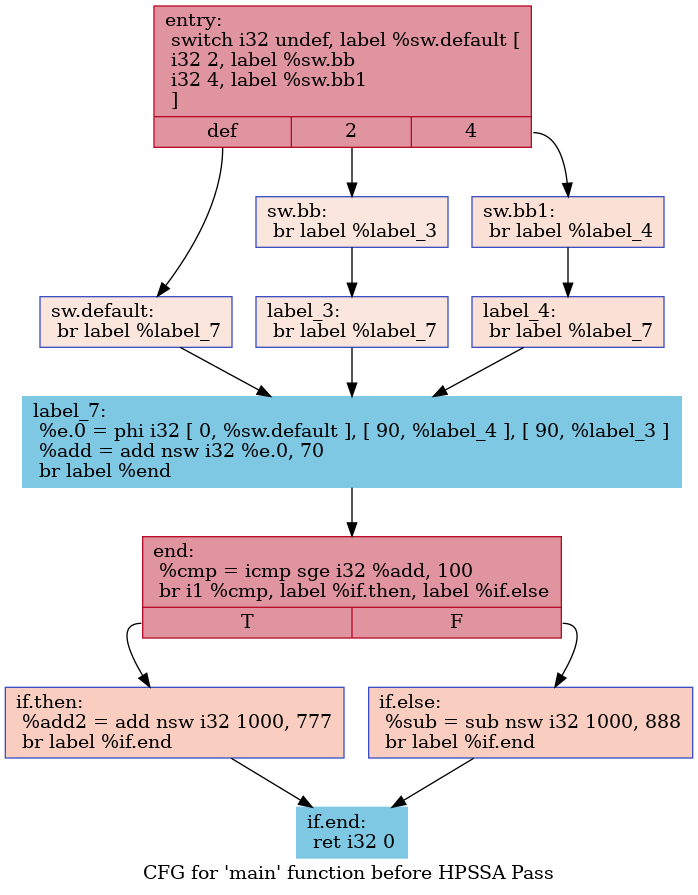
\includegraphics[width=5.3cm,height=7.5cm]{baseline.dot.png}
	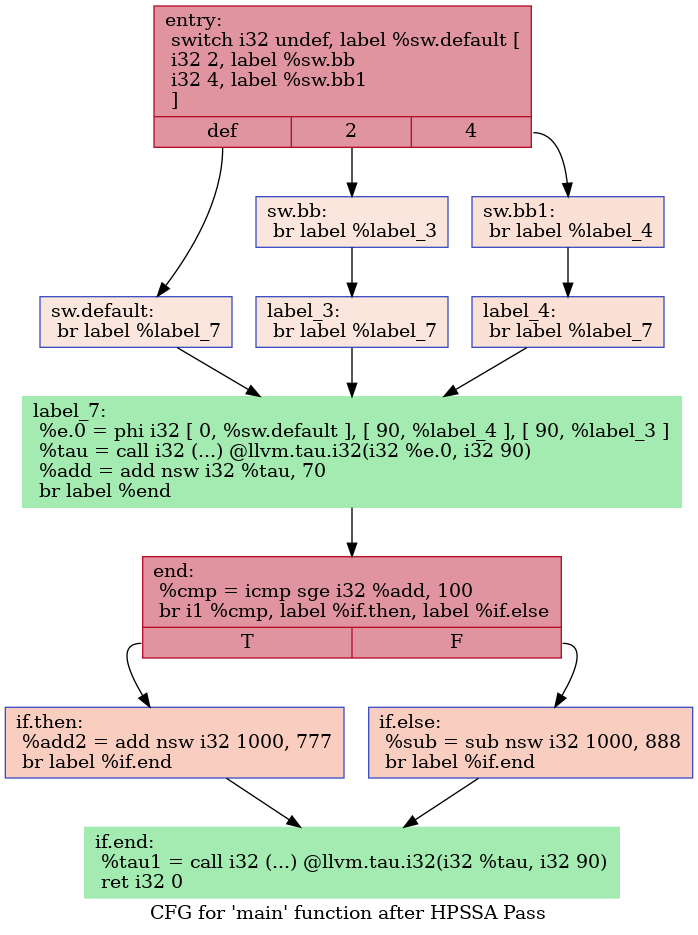
\includegraphics[width=5.3cm,height=7.5cm]{afterHPSSA.dot.png}
\end{frame}

\begin{frame}
	\frametitle{\texttt{HPSSAPass} : Main Pass}
	\begin{itemize}
		\item \mintinline[fontsize=\footnotesize]{css}{HPSSAPass::run(Function \&F, FunctionAnalysisManager \&AM)} 
		\begin{itemize}
			\footnotesize
			\item Invoke \mintinline[fontsize=\footnotesize]{css}{HPSSAPass::getProfileInfo()} function to get a compact representation of all the profiled \color{red} hot paths \color{black} in the program and then call \mintinline[fontsize=\footnotesize]{css}{HPSSAPass::getCaloricConnector()} to get all the caloric connectors from the \color{red} hot path \color{black} information. This is a precursor to finding strategic positions to place \mintinline[]{css}{"llvm.tau"} intrinsic calls in the LLVM IR.
			\item Runs over each basic block in the function "F" in topological order using iterator returned from \mintinline[fontsize=\footnotesize]{css}{llvm::Function::RPOT()} call.
			\item Uses the \mintinline[fontsize=\footnotesize]{css}{llvm::dominates()} function from \mintinline[fontsize=\footnotesize]{css}{llvm::DominatorTreeAnalysis} to check for dominance frontier while processing the child nodes of the current basic block. This step is a part of correctly placing \mintinline[]{css}{"llvm.tau"} intrinsic calls in the LLVM IR. 
			\item Uses the renaming stack and \mintinline[]{css}{HPSSAPass::Search()} function to search and replace all use of PHI result operand with that returned by the \mintinline[]{css}{"llvm.tau"} intrinsic call.
		\end{itemize}
	\end{itemize}
\end{frame}

\begin{frame}
	\frametitle{\texttt{HPSSAPass} : Destruction Pass}
	\begin{itemize}
		\item Out of HPSSA Form. 
		\begin{itemize}
			\item A seperate pass using the new LLVM Pass Manager. \mintinline[]{css}{class TDSTRPass : public PassInfoMixin<TDSTRPass>}
			\item Using \mintinline[fontsize=\footnotesize]{css}{TDSTRPass::run(Function \&F, ...)}, we replace all use of existing tau operands with first argument of  \mintinline[]{css}{"llvm.tau"} intrinsic (corresponds to the safe argument) and remove the \mintinline[]{css}{"llvm.tau"} intrinsic calll from the LLVM IR.
			\item The LLVM IR becomes identical to what it was before running the HPSSA Pass. 
		\end{itemize}
	\end{itemize}
\end{frame}

\begin{frame}[fragile]
	\frametitle{\texttt{HPSSAPass} : Usage [It is easy!]}
	\begin{itemize}
		\item Include \mintinline[]{css}{llvm::HPSSAPass} header file.
		\item Load shared object using opt tool. \mintinline[]{css}{opt -load HPSSA.cpp.so ...} 
	\end{itemize}
	\begin{minted}[fontsize=\tiny, tabsize=2, highlightlines={1,14,15,18}, linenos]{cpp}
	#include <HPSSA.h> // import the header.
	
	class MyExamplePass : public PassInfoMixin<MyExamplePass> {
		public: PreservedAnalyses run(Function &F, 
			FunctionAnalysisManager &AM);
	};
	...
	
	PreservedAnalyses MyExamplePass::run(Function &F, 
		FunctionAnalysisManager &AM) {
		if (F.getName() != "main")
			return PreservedAnalyses::all();
	
		HPSSAPass hpssaUtil; // Make a HPSSAPass Object.
		hpssaUtil.run(F, AM);  // Call the HPSSAPass::run() function.
	
		std::vector<Instruction *> TauInsts 
			= hpssaUtil.getAllTauInstrunctions(F); // Calling HPSSA utility function.
			
		std::cout << "\t\tTotal Tau Instructions : " << TauInsts.size() << "\n";
		...
	}
	
	/// [output] Total Tau Instructions : 7 
	\end{minted}
\end{frame}

\section{SSCCP Pass in LLVM}

\begin{frame}
	\frametitle{New Additions to SCCP Pass}
	\begin{itemize}
		\item We implement a speculative version of the SCCP to demonstrate the usefulness of the HPSSA Form.
		\item Modified the existing SCCP Pass to add in \mintinline[fontsize=\footnotesize]{css}{SCCPInstVisitor::visitTauNode()} function similar to \mintinline[fontsize=\footnotesize]{css}{SCCPInstVisitor::visitPHINode()}, which handles the special \mintinline[fontsize=\footnotesize]{css}{"llvm.tau"} intrinsic instructions added for $\tau$-functions.
		\item Added a new lattice element type \mintinline[fontsize=\footnotesize]{css}{"spec_constant"} in \mintinline[fontsize=\footnotesize]{css}{ValueLattice} class supporting operations on speculative constants. 
		\item Added new functions in the \mintinline[fontsize=\footnotesize]{css}{SCCPInstVisitor} and \mintinline[fontsize=\footnotesize]{css}{SCCPSolver} class to handle operations on speculative constants. Eg. Operands can be marked speculative using \mintinline[fontsize=\footnotesize]{css}{markSpeculativeConstant()} function.
	\end{itemize}
\end{frame}

\begin{frame}[fragile]
	\frametitle{Further Modifications}
	\begin{itemize}
		\item Modified the \mintinline[fontsize=\footnotesize]{css}{SCCPInstVisitor::mergeIn()} function to handle lattice ''meet" operation for the new speculative constants introduced.  
		\item Since we added the $\tau$-functions as an \mintinline[fontsize=\footnotesize]{css}{"llvm.tau"} intrinsic which is essentially an \mintinline[fontsize=\footnotesize]{css}{llvm:CallInst} type, we modified all appropriate visit and marking functions in \mintinline[fontsize=\footnotesize]{css}{SCCPInstVisitor, SCCPSolver} and \mintinline[fontsize=\footnotesize]{css}{SCCPPass} to handle this case separately by calling \mintinline[fontsize=\footnotesize]{css}{visitTauNode()}.
		\item Modified utility functions in \mintinline[fontsize=\footnotesize]{css}{SCCPInstVisitor} and \mintinline[fontsize=\footnotesize]{css}{SCCPSolver} class to print marking of speculative constants and related operations for debugging purpose.
	\end{itemize}
\begin{minted}[fontsize=\tiny, tabsize=2, highlightcolor=lime, linenos, highlightlines={4,5,8}]{css}
... // logs
[BBWorkList] Visiting LLVM Instrinsic : llvm.tau (call)
	Visiting Tau Instruction
		Speculative Operand : , speculative constant
		Speculative Operand : llvm.tau.i32, speculative constant
	Merged speculative constant into   %tau = call i32 (...) 
		@llvm.tau.i32(i32 %e.0, i32 90) : speculative constant
	ValueLattice (TauState) : speculative constant
...
\end{minted}
\end{frame}
\footnotesize
\begin{frame}[fragile]
	\frametitle{SSCCP with an Example}
We run the speculative SCCP on the example below.
\begin{columns}
	\begin{column}{0.2\textwidth}
\begin{minted}[fontsize=\tiny, tabsize=2, linenos, highlightcolor=yellow, highlightlines={16,20}]{cpp}
int main() {
	int a = 1000, z, c, e = 0;
	switch(c) {   
		case 2 : goto label_3; break;
		case 4 : goto label_4; break;
		default : goto label_7; 
	}
	label_3:
		e = 90;
		goto label_7;
	label_4:
		e = 100 - 10;
		goto label_7;
	label_7:
	// e in rhs is 90.
		e = e + 70;  
		goto end;
	end:
	// e is greater than 100 always
		if (e >= 100) {  
			a = a + 777;
		} else {
			a = a - 888;
		} return 0; 
}
\end{minted}
	\end{column}
	\begin{column}{0.5\textwidth}  
		\begin{center}
			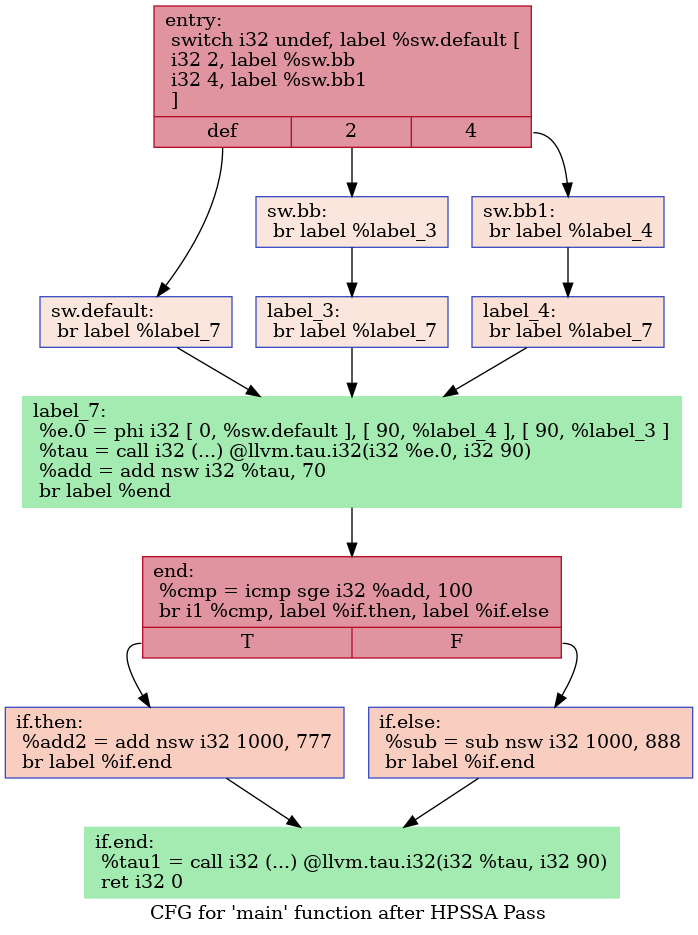
\includegraphics[width=4.5cm,height=6.5cm]{afterHPSSA.dot.png}
		\end{center}
	\end{column}
\end{columns}
\end{frame}

\begin{frame}
	\frametitle{SSCCP with an Example}
	\footnotesize
	\begin{itemize}
\item The \textsc{PHINode} at \texttt{label\_7} is removed due to constant propagation of value 90 for variable "e" along all paths. However since the operands of the $\tau$-function are marked speculative, this instruction and it's uses are not removed by the SSCCP Pass.
	\end{itemize}
	\centering
	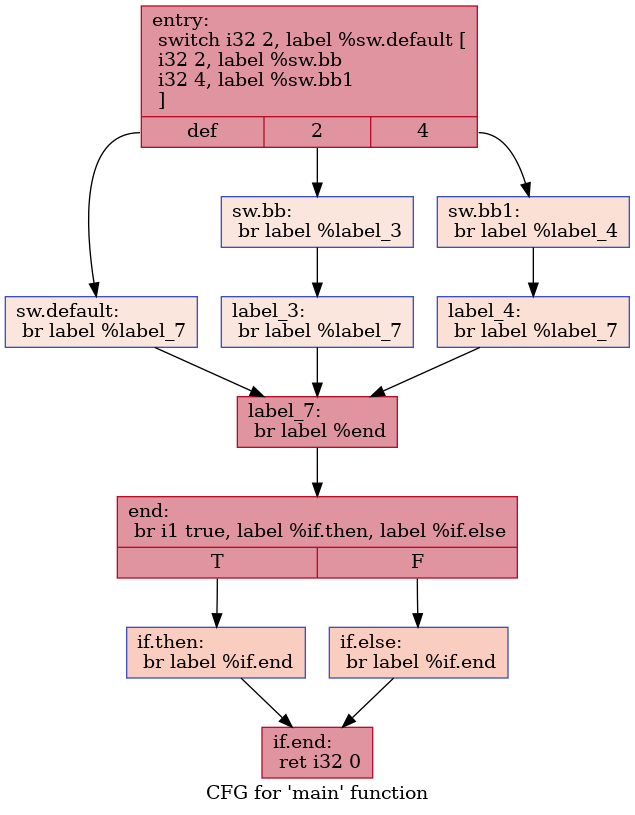
\includegraphics[width=4.6cm,height=6.1cm]{SCCP_BASELINE.dot.png}
	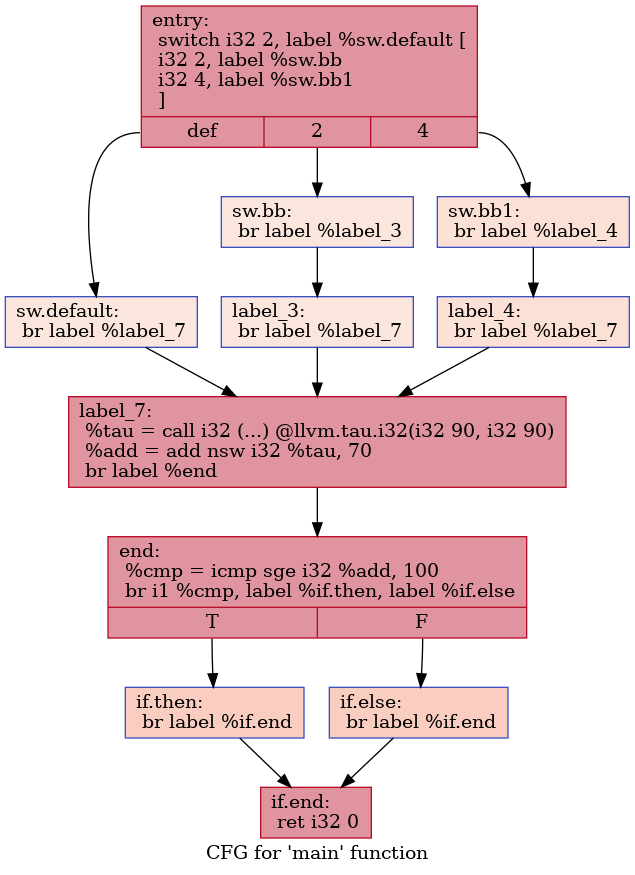
\includegraphics[width=4.6cm,height=6.1cm]{specSCCP_HPSSA.dot.png}
\end{frame}

\end{document}